\documentclass[b4paper, landscape, dvipdfmx]{jsarticle}
%----- 必要なパッケージ -----
\usepackage{fancybox,ascmac,otf}
\usepackage{amssymb, amsthm}
\usepackage[leqno]{amsmath}
\usepackage{geometry}
\usepackage{multicol}
\usepackage{tcolorbox}
\usepackage{xcolor}
\usepackage{fancyhdr}
\usepackage{tikz}

% TikZライブラリ
\usetikzlibrary{
    positioning,
    arrows.meta,
    calc,
    shadows,
    shadows.blur,
    intersections,
    angles,
    quotes,
    decorations.pathmorphing,
    patterns
}

% tcolorboxライブラリ
\tcbuselibrary{skins, breakable, theorems}

\usepackage{enumitem}
\setlist[enumerate,1]{label=(\arabic*)}
\setlist[itemize]{leftmargin=*}
\newcommand{\ds}{\displaystyle}

%----- レイアウト設定 -----
\geometry{
  left=15mm,
  right=15mm,
  top=20mm,
  bottom=15mm,
  headheight=25pt
}

%----- 数式環境の上下の余白調整 -----
\AtBeginDocument{
  \setlength{\abovedisplayskip}{5pt}
  \setlength{\belowdisplayskip}{5pt}
  \setlength{\abovedisplayshortskip}{0pt}
  \setlength{\belowdisplayshortskip}{3pt}
}

%===========================================================
%  デザイン設定
%===========================================================

%--- 色の定義 ---
\definecolor{printBlue}{RGB}{0, 50, 100}     % 濃紺
\definecolor{printRed}{RGB}{140, 20, 20}     % 濃エンジ
\definecolor{printTeal}{RGB}{0, 60, 60}      % 濃い青緑
\definecolor{fillOrange}{RGB}{255, 230, 200} % 領域塗りつぶし用

%--- 共通スタイル定義 ---
\tcbset{
    chartbox/.style={
        enhanced,
        fonttitle=\sffamily\bfseries,
        boxrule=1pt,
        arc=2pt,
        top=1.0em,
        nobeforeafter,
        enlarge left by=-2mm,
        enlarge right by=-2mm,
        drop fuzzy shadow,
        colback=white,
        attach boxed title to top left={xshift=10pt, yshift*=-\tcboxedtitleheight/2},
        boxed title style={frame hidden, sharp corners, rounded corners=southeast, arc=3pt}
    }
}

%--- 各種ボックス環境定義 ---
\newtcolorbox{any}[1]{
    enlarge left by=0mm, enlarge right by=0mm,
    enhanced, frame hidden, colback=white, title={#1},
    attach boxed title to top left={xshift=0mm, yshift=0mm},
    coltitle=white, fonttitle=\bfseries\sffamily,
    boxed title style={
        colback=black!80, frame hidden, arc=4pt, outer arc=4pt,
        sharp corners=south, boxrule=0pt,
        top=1mm, bottom=1mm, left=3mm, right=3mm
    },
    underlay boxed title={
        \draw[thick, black!80] (title.south west) -- (title.south west-|frame.east);
    },
    breakable, top=5mm, left=2mm, right=2mm, bottom=0mm,
    before skip=1em, after skip=1em,
    segmentation style={draw=black!40, dashed}
}

\newtcolorbox{eg}[1]{
    chartbox,
    colframe=printBlue,
    coltitle=white,
    title=\textbf{例題 #1},
    boxed title style={colback=printBlue},
    segmentation style={draw=printBlue, line width=0.5pt, dashed}
}

\newtcolorbox{prac}[1]{
    chartbox,
    colframe=printRed,
    coltitle=white,
    title=\textbf{練習 #1},
    boxed title style={colback=printRed}
}

\newtcolorbox{thm}[1]{
    chartbox,
    colframe=printTeal,
    coltitle=white,
    title=\textbf{#1},
    boxed title style={colback=printTeal}
}

\newtcolorbox{answer}[1][height fill]{
    enhanced,
    title={Memo / Answer},
    colframe=black!80,
    colback=white,
    coltitle=black!60,
    fonttitle=\sffamily\bfseries,
    attach boxed title to top left={xshift=5mm, yshift*=-\tcboxedtitleheight/2},
    boxed title style={frame hidden, colback=white},
    boxrule=1pt,
    arc=1pt,
    nobeforeafter,
    enlarge left by=-2mm, 
    enlarge right by=-2mm, 
    height fill,
    segmentation style={draw=black!20, solid},
    underlay={
        \begin{tcbclipinterior}
            \draw[step=5mm, black!5, ultra thin] (interior.south west) grid (interior.north east);
        \end{tcbclipinterior}
    }, 
    #1
}

%----- ヘッダーの設定 -----
\pagestyle{fancy}
\fancyhf{}
\fancyhead[C]{%
    \begin{tikzpicture}[remember picture, overlay]
        \node[anchor=north west, fill=printBlue, minimum width=\paperwidth, minimum height=5pt] at (current page.north west) {};
    \end{tikzpicture}
}
\fancyhead[L]{\small \textcolor{black!90}{数学C $>$ 第1章--平面ベクトル $>$ 第13回 \textbf{点の存在範囲}}}
\fancyhead[R]{\small 年 \hspace{1cm} 組 \hspace{1cm} 番 \quad 氏名 \hspace{6cm}}
\renewcommand{\headrulewidth}{0pt}

\begin{document}

%=============================================================================
% 1枚目:基本パターンの可視化
%=============================================================================
\begin{multicols}{2}

%-----------------------------------------------------------------------------
% 左カラム:係数と領域
%-----------------------------------------------------------------------------
\begin{any}{1. 係数が動くと, 点も動く}
    $\overrightarrow{\text{OP}} = s\vec{a} + t\vec{b}$ という式において, 係数 $s, t$ がある条件を満たしながら変化するとき, 点 P はどのような図形を描くだろうか.
    
    \begin{thm}{基本の3パターン}
        $\triangle$OAB において, $\overrightarrow{\text{OP}} = s\vec{a} + t\vec{b}$ とする.
        
        \begin{enumerate}
            \item \textbf{直線AB}:
            \[ s + t = 1 \]
            \item \textbf{三角形OABの周と内部}:
            \[ 0 \leqq s+t \leqq 1, \quad s \geqq 0, \quad t \geqq 0 \]
            \item \textbf{平行四辺形の周と内部}:
            \[ 0 \leqq s \leqq 1, \quad 0 \leqq t \leqq 1 \]
        \end{enumerate}
    \end{thm}
    
    \textbf{イメージ図:}
    \begin{center}
    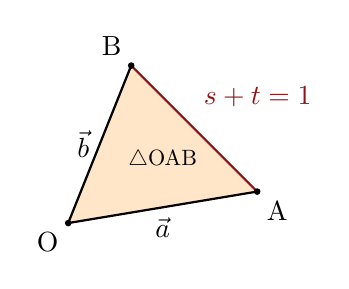
\begin{tikzpicture}[scale=0.8, >=stealth]
        % 座標設定
        \coordinate (O) at (0,0);
        \coordinate (A) at (3,0.5);
        \coordinate (B) at (1,2.5);
        \coordinate (C) at ($(A)+(B)$); % 平行四辺形の頂点
        
        % パターン2: 三角形
        \fill[fillOrange] (O)--(A)--(B)--cycle;
        \draw[thick] (O)--(A) node[midway, below]{$\vec{a}$};
        \draw[thick] (O)--(B) node[midway, left]{$\vec{b}$};
        \draw[thick, printRed] (A)--(B);
        
        \node[scale=0.8] at (1.5, 1) {$\triangle$OAB};
        \node[printRed, right] at (2, 2) {$s+t=1$};
        
        \fill (O) circle (1.5pt) node[below left]{O};
        \fill (A) circle (1.5pt) node[below right]{A};
        \fill (B) circle (1.5pt) node[above left]{B};
    \end{tikzpicture}
    \hspace{0.5cm}
    \begin{tikzpicture}[scale=0.8, >=stealth]
        % 座標設定
        \coordinate (O) at (0,0);
        \coordinate (A) at (3,0.5);
        \coordinate (B) at (1,2.5);
        \coordinate (C) at ($(A)+(B)$);
        
        % パターン3: 平行四辺形
        \fill[fillOrange] (O)--(A)--(C)--(B)--cycle;
        \draw[dashed] (A)--(C)--(B);
        \draw[thick] (O)--(A);
        \draw[thick] (O)--(B);
        
        \node[scale=0.8] at (2, 1.5) {平行四辺形};
        \node[align=left, scale=0.7] at (2, -0.8) {$0 \leqq s \leqq 1$\\$0 \leqq t \leqq 1$};
        
        \fill (O) circle (1.5pt) node[below left]{O};
        \fill (A) circle (1.5pt);
        \fill (B) circle (1.5pt);
    \end{tikzpicture}
    \end{center}
    
    特に重要なのは \textbf{(1) $s+t=1$} である. これが「直線」を表す条件となる.
\end{any}

\columnbreak

\begin{any}{2. 「ななめの座標」で考える(斜交座標)}
    第2回で触れた通り, $\vec{a}$ と $\vec{b}$ を基準にすると, 平面上に\textbf{斜めのマス目(グリッド)}を作ることができる.
    \[ \vec{p} = s\vec{a} + t\vec{b} \iff \text{点 P の座標は } (s, t) \]
    この視点で見れば, 難しいベクトルの式も, 中学・高1で習った「グラフ」と同じに見えてくる.

    \begin{thm}{いつものグラフと比較}
        \begin{itemize}
            \item \textbf{直線 AB}: $s + t = 1$ $\iff$ 直交座標の直線 $x + y = 1$
            \item \textbf{平行四辺形の内部}: $0 \leqq s, t \leqq 1$ $\iff$ 直交座標の正方形 $0 \leqq x, y \leqq 1$
        \end{itemize}
    \end{thm}
    
    \begin{center}
    % 左側:斜交座標(ベクトル)
    \begin{minipage}[t]{0.48\linewidth}
        \centering
        \textbf{【ベクトルの世界】} \\ \small (軸が歪んでいる)
        \vspace{5pt}
        \begin{tikzpicture}[scale=0.8, >=stealth]
            % 座標設定
            \coordinate (O) at (0,0);
            \coordinate (A) at (2.5, 0.5);
            \coordinate (B) at (1, 2);
            
            % 斜交グリッド
            \clip (-1, -1) rectangle (4.5, 3.5);
            \foreach \s in {-1, 0, ..., 2} {
                \draw[gray!70, thin] ($(O)+\s*(A)-(B)$) -- ($(O)+\s*(A)+2*(B)$);
            }
            \foreach \t in {-1, 0, ..., 2} {
                \draw[gray!70, thin] ($(O)+\t*(B)-(A)$) -- ($(O)+\t*(B)+2*(A)$);
            }
            
            % 軸ベクトル
            \draw[->, thick, printBlue] (O)--(A) node[below right]{$\vec{a}$};
            \draw[->, thick, printBlue] (O)--(B) node[above left]{$\vec{b}$};
            \fill (O) circle (2pt) node[below left]{O};
            
            % 直線 s+t=1 (AとBを通る直線)
            % shortenにマイナスを指定して延長
            \draw[very thick, printRed, shorten <=-2cm, shorten >=-2cm] (A) -- (B);
            \node[printRed, fill=white, inner sep=1pt, scale=0.8] at (2.5, 2.5) {$s+t=1$};
            
            % 平行四辺形領域
            \coordinate (C) at ($(A)+(B)$);
            \fill[fillOrange, opacity=0.6] (O)--(A)--(C)--(B)--cycle;
            \node[scale=0.7] at (1.8, 1.2) {領域};
        \end{tikzpicture}
    \end{minipage}
    \hfill
    % 右側:直交座標(xy平面)
    \begin{minipage}[t]{0.48\linewidth}
        \centering
        \textbf{【いつもの$xy$世界】} \\ \small (軸が直角)
        \vspace{5pt}
        \begin{tikzpicture}[scale=0.8, >=stealth]
            % 座標設定 (単位ベクトルを少し大きめに取る)
            \coordinate (O) at (0,0);
            \coordinate (X) at (2, 0); % (1,0)
            \coordinate (Y) at (0, 2); % (0,1)
            
            % 直交グリッド
            \draw[step=2, gray!70, thin] (-1,-1) grid (4.5, 3.5);
            \draw[->, gray] (-0.5, 0) -- (4, 0) node[right]{$x$};
            \draw[->, gray] (0, -0.5) -- (0, 3.5) node[above]{$y$};
            
            % 単位ベクトル的な点
            \fill (X) circle (2pt) node[below right]{$1$};
            \fill (Y) circle (2pt) node[above left]{$1$};
            \fill (O) circle (2pt) node[below left]{O};
            
            % 直線 x+y=1
            \draw[very thick, printRed, shorten <=-2cm, shorten >=-2cm] (X) -- (Y);
            \node[printRed, fill=white, inner sep=1pt, scale=0.8] at (3, 2) {$x+y=1$};
            
            % 正方形領域
            \coordinate (XY) at (2, 2);
            \fill[fillOrange, opacity=0.6] (O)--(X)--(XY)--(Y)--cycle;
            \node[scale=0.7] at (1, 1) {領域};
        \end{tikzpicture}
    \end{minipage}
    \end{center}
    
    \textbf{結論:} ベクトルの係数 $s, t$ は, 斜めの世界での座標 $(x, y)$ だと思えばよい.
\end{any}

%-----------------------------------------------------------------------------
% 右カラム:変形テクニック
%-----------------------------------------------------------------------------
\columnbreak

\begin{any}{3. 「和を1にする」テクニック}
    もし $s+t=2$ のようになったらどうするか?
    ベクトルの世界では\textbf{「係数の和が1」}の形に持ち込むのが鉄則である.
    
    \begin{itemize}
        \item 式全体を割って, 右辺を無理やり 1 にする.
        \item 係数を調整して, 新しい基底ベクトル(矢印)を作る.
    \end{itemize}

    \begin{eg}{1 (基本変形)}
        $\triangle$OAB において, $\overrightarrow{\text{OP}} = s\vec{a} + t\vec{b}$ とする.
        $s + t = 2$ を満たすとき, 点 P の存在範囲を図示せよ.
        
        \tcblower
        \textbf{手順:}
        1. 両辺を 2 で割る. $\ds \frac{s}{2} + \frac{t}{2} = 1$.
        2. $\ds s' = \frac{s}{2}, t' = \frac{t}{2}$ と置く. ($s'+t'=1$)
        3. 元の式を $s', t'$ で書き換える.
           \[ \vec{p} = s\vec{a} + t\vec{b} = (2s')\vec{a} + (2t')\vec{b} = s'(2\vec{a}) + t'(2\vec{b}) \]
        4. 新しい矢印 $2\vec{a}, 2\vec{b}$ の終点を結ぶ直線を考える.
        
        \begin{center}
        \begin{tikzpicture}[scale=0.7, >=stealth]
            \coordinate (O) at (0,0);
            \coordinate (A) at (2,0.5);
            \coordinate (B) at (0.5,1.5);
            \coordinate (A2) at (4,1); % 2a
            \coordinate (B2) at (1,3); % 2b
            
            \draw[->, gray] (O)--(A) node[midway, below]{$\vec{a}$};
            \draw[->, gray] (O)--(B) node[midway, left]{$\vec{b}$};
            \draw[->, thick, printBlue] (O)--(A2) node[below right]{A$'$($2\vec{a}$)};
            \draw[->, thick, printBlue] (O)--(B2) node[above left]{B$'$($2\vec{b}$)};
            
            \draw[thick, printRed] (A2)--(B2);
            \fill (A2) circle (2pt); \fill (B2) circle (2pt);
            
            \node[printRed] at (3, 2.5) {Pの範囲};
        \end{tikzpicture}
        \end{center}
        \vspace{8cm}
    \end{eg}
\end{any}

\columnbreak

%-----------------------------------------------------------------------------
% 左カラム:不等式の場合
%-----------------------------------------------------------------------------
\begin{any}{4. 不等式になってもやることは同じ}
    条件が $s+t \leqq 2$ のように不等式になった場合も, 同様に変形する.
    
    \begin{eg}{2 (不等式の領域)}
        $\triangle$OAB において, $\overrightarrow{\text{OP}} = s\vec{a} + t\vec{b}$ とする.
        $2s + 3t \leqq 1, \quad s \geqq 0, \quad t \geqq 0$
        のとき, 点 P の存在範囲を図示せよ.
        
        \tcblower
        \textbf{手順:}
        1. 右辺は既に 1 なので, 左辺を無理やり $(s') + (t') \leqq 1$ の形と見る.
           \[ 2s + 3t = (2s) + (3t) \leqq 1 \]
        2. $s' = 2s, \ t' = 3t$ と置く. ($s' \geqq 0, t' \geqq 0$)
        3. 元の式を書き換える.
           $s = \frac{1}{2}s', \ t = \frac{1}{3}t'$ なので,
           \[ \vec{p} = \frac{1}{2}s'\vec{a} + \frac{1}{3}t'\vec{b} = s'(\frac{1}{2}\vec{a}) + t'(\frac{1}{3}\vec{b}) \]
        4. 新しい矢印 $\frac{1}{2}\vec{a}, \frac{1}{3}\vec{b}$ で作られる三角形を描く.
        \vspace{12cm}
    \end{eg}
\end{any}

%-----------------------------------------------------------------------------
% 右カラム:直交座標との類似
%-----------------------------------------------------------------------------

\end{multicols}

%=============================================================================
% 3枚目:確認テスト(問題)
%=============================================================================
\newpage
\fancyhead[L]{\small \textcolor{black!90}{数学C $>$ 第1章--平面ベクトル $>$ 第13回--\textbf{確認テスト}}}
\begin{multicols}{2}

\begin{any}{確認テスト (A: 基本)}
    \begin{prac}{A1 (直線の変形)}
        $\triangle$OAB において, $\overrightarrow{\text{OP}} = s\vec{a} + t\vec{b}$ とする.
        次の条件を満たす点 P の存在範囲を答えよ(「どのような図形か」を言葉で記述し, 図示せよ).
        \[ 2s + t = 1 \]
    \end{prac}
    \begin{answer}[height=6cm]
        \begin{center}
        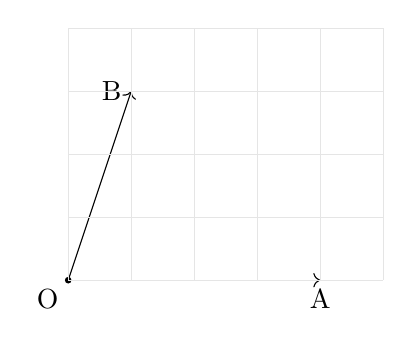
\begin{tikzpicture}[scale=0.8]
            \coordinate (O) at (0,0);
            \coordinate (A) at (4,0);
            \coordinate (B) at (1,3);
            \draw[->] (O)--(A) node[below]{A};
            \draw[->] (O)--(B) node[left]{B};
            \fill (O) circle (1.5pt) node[below left]{O};
            % グリッド線
            \draw[gray!20] (0,0) grid (5,4);
        \end{tikzpicture}
        \end{center}
    \end{answer}

    \begin{prac}{A2 (領域の変形)}
        条件が以下のとき, 点 P の存在範囲を図示せよ.
        \[ s + t \leqq 2, \quad s \geqq 0, \quad t \geqq 0 \]
    \end{prac}
    \begin{answer}[height=6cm]
    \end{answer}
\end{any}

\columnbreak

\begin{any}{確認テスト (B: 標準)}
    \begin{prac}{B1 (一般形の領域)}
        $\triangle$OAB において, $\overrightarrow{\text{OP}} = s\vec{a} + t\vec{b}$ とする.
        \[ 2s + 3t \leqq 6, \quad s \geqq 0, \quad t \geqq 0 \]
        を満たす点 P の存在範囲を図示し, その面積は $\triangle$OAB の面積の何倍か求めよ.
    \end{prac}
    \begin{answer}[height=14cm]
        \textbf{図示:}
        \vspace{4cm}
        \\
        \textbf{面積比の計算:}
    \end{answer}
\end{any}

\end{multicols}

%=============================================================================
% 4枚目:確認テスト(解答)
%=============================================================================
\newpage
\fancyhead[L]{\small \textcolor{black!90}{数学C $>$ 第1章--平面ベクトル $>$ 第13回 \textbf{【解答解説】}}}

\begin{multicols}{2}

\begin{any}{解答 (A: 基本)}
    \begin{prac}{A1 解答}
        式を変形する: $(2s) + t = 1$.
        $\vec{p} = s\vec{a} + t\vec{b} = (2s)(\frac{1}{2}\vec{a}) + t\vec{b}$.
        
        よって, 辺OAの中点($\frac{1}{2}\vec{a}$)を A$'$, 点Bを B$'$($\vec{b}$) としたとき,
        \textbf{直線 A$'$B$'$} が求める範囲である.
        
        (補足: 直線AB上の点ではなく, 線分OAの中点とBを通る直線になる)
    \end{prac}

    \begin{prac}{A2 解答}
        両辺を 2 で割る: $\frac{s}{2} + \frac{t}{2} \leqq 1$.
        式は $\vec{p} = (\frac{s}{2})(2\vec{a}) + (\frac{t}{2})(2\vec{b})$.
        
        OAを2倍に延長した点を A$'$, OBを2倍に延長した点を B$'$ とする.
        求める範囲は, $\mathbf{\triangle OA'B'}$ \textbf{の周と内部}である.
    \end{prac}
\end{any}

\columnbreak

\begin{any}{解答 (B: 標準)}
    \begin{prac}{B1 解答}
        両辺を 6 で割って右辺を 1 にする.
        \[ \frac{2s}{6} + \frac{3t}{6} \leqq 1 \iff \frac{s}{3} + \frac{t}{2} \leqq 1 \]
        
        これを $\vec{p}$ の式に反映させるには,
        \[ \vec{p} = s\vec{a} + t\vec{b} = \frac{s}{3}(3\vec{a}) + \frac{t}{2}(2\vec{b}) \]
        と変形する.
        
        \textbf{図形の特定:}
        \begin{itemize}
            \item A$'$: OAを3倍に延長した点 ($3\vec{a}$)
            \item B$'$: OBを2倍に延長した点 ($2\vec{b}$)
        \end{itemize}
        これらで作られる $\triangle$OA$'$B$'$ の周と内部が求める範囲.
        
        \textbf{面積比:}
        底辺(OA方向)が 3倍, 高さ方向(OB方向)が 2倍 になっているので,
        面積は $3 \times 2 = 6$ 倍.
        
        \textbf{答え:} $\triangle$OAB の \textbf{6倍}
    \end{prac}
\end{any}

\end{multicols}
\end{document}